% Dario's website evaluation 
\section{Dario's Evaluation}
\subsection{Scores}
Outlined below are the evaluations provided by Dario Crippa for the Nielsen and MiLe heuristics carefully selected by the group to analyze the website.\\
% Nielsen's Heuristics Evaluation
\begin{table}[htp!]
    \centering
    \begin{tabular}{ |l|l|c| }
        \hline
        \textbf{Code} & \textbf{Description} & \textbf{Score}\\
        \hline
        \textbf{H1} & Visibility of system status & \textbf{\color{unicefOrange}{3}}\\
        \hline
        \textbf{H2} & Match between system and the real world & \textbf{\color{unicefGreen}{5}}\\
        \hline
        \textbf{H3} & User control and freedom & \textbf{\color{unicefRed}{2}}\\
        \hline
        \textbf{H4} & Consistency and standards & \textbf{\color{unicefGreen}{5}}\\
        \hline
        \textbf{H5} & Error prevention & \textbf{\color{unicefGreen}{4}}\\
        \hline
        \textbf{H6} & Recognition rather than recall & \textbf{\color{unicefGreen}{5}}\\
        \hline
        \textbf{H7} & Flexibility and efficiency of use & \textbf{\color{unicefOrange}{3}}\\
        \hline
        \textbf{H8} & Aesthetic and minimalist design & \textbf{\color{unicefOrange}{3}}\\
        \hline
        \textbf{H9} & Help users recognize, diagnose and recover from errors & \textbf{\color{unicefGray}{n.a}}\\
        \hline
        \textbf{H10} & Help and documentation & \textbf{\color{unicefGreen}{4}}\\
        \hline
    \end{tabular}
    \caption{\textbf{Nielsen}'s heuristics scores}
\end{table}
% MiLe Heuristics Evaluation
\begin{table}[htp!]
    \centering
    \begin{tabular}{ |c|l|l|c| }
        \hline
        \textbf{Group} & \textbf{Code} & \textbf{Description} & \textbf{Score}\\
        \hline
        \multirow{5}{*}{\textbf{Navigation}} & \textbf{M1} & Interaction consistency & \textbf{\color{unicefRed}{2}}\\
        \cline{2-4}
        & \textbf{M2} & Group navigation & \textbf{\color{unicefGreen}{4}}\\
        \cline{2-4}
        & \textbf{M3} & Navigation support & \textbf{\color{unicefGreen}{4}}\\
        \cline{2-4}
        & \textbf{M4} & User control & \textbf{\color{unicefOrange}{3}}\\
        \cline{2-4}
        & \textbf{M5} & Error prevention & \textbf{\color{unicefGreen}{4}}\\
        \hline
        \textbf{Content} & \textbf{M6} & Information overload & \textbf{\color{unicefOrange}{3}}\\
        \hline
        \multirow{6}{*}{\textbf{Presentation}} & \textbf{M7} & Text layout & \textbf{\color{unicefGreen}{5}}\\
        \cline{2-4}
        & \textbf{M8} & Interaction placeholder semiotics & \textbf{\color{unicefGreen}{4}}\\
        \cline{2-4}
        & \textbf{M9} & Interaction placeholder consistency & \textbf{\color{unicefGreen}{4}}\\
        \cline{2-4}
        & \textbf{M10} & Spatial allocation & \textbf{\color{unicefOrange}{3}}\\
        \cline{2-4}
        & \textbf{M11} & Consistency of the page structure & \textbf{\color{unicefGreen}{4}}\\
        \cline{2-4}
        & \textbf{M12} & Coherence in page layout & \textbf{\color{unicefGreen}{5}}\\
        \hline
    \end{tabular}
    \caption{\textbf{MiLe} heuristics scores}
\end{table}
% Comments 
\newpage
\subsection{Comments}
This section offers clear and concise explanations and justifications for the scores assigned to the previously presented heuristics.
% Nielsen's Heuristics Comments
\subsubsection{Nielsen's Heuristics}
\begin{description}
    \item {\textbf{H1} \color{unicefGray}{Visibility of the system status}}\\
    While breadcrumbs (1) provide clear and intuitive navigation in some sections, other areas feel a bit chaotic. 
    There are moments where users might feel a bit lost (2).
    \begin{figure}[h]
        \centering
        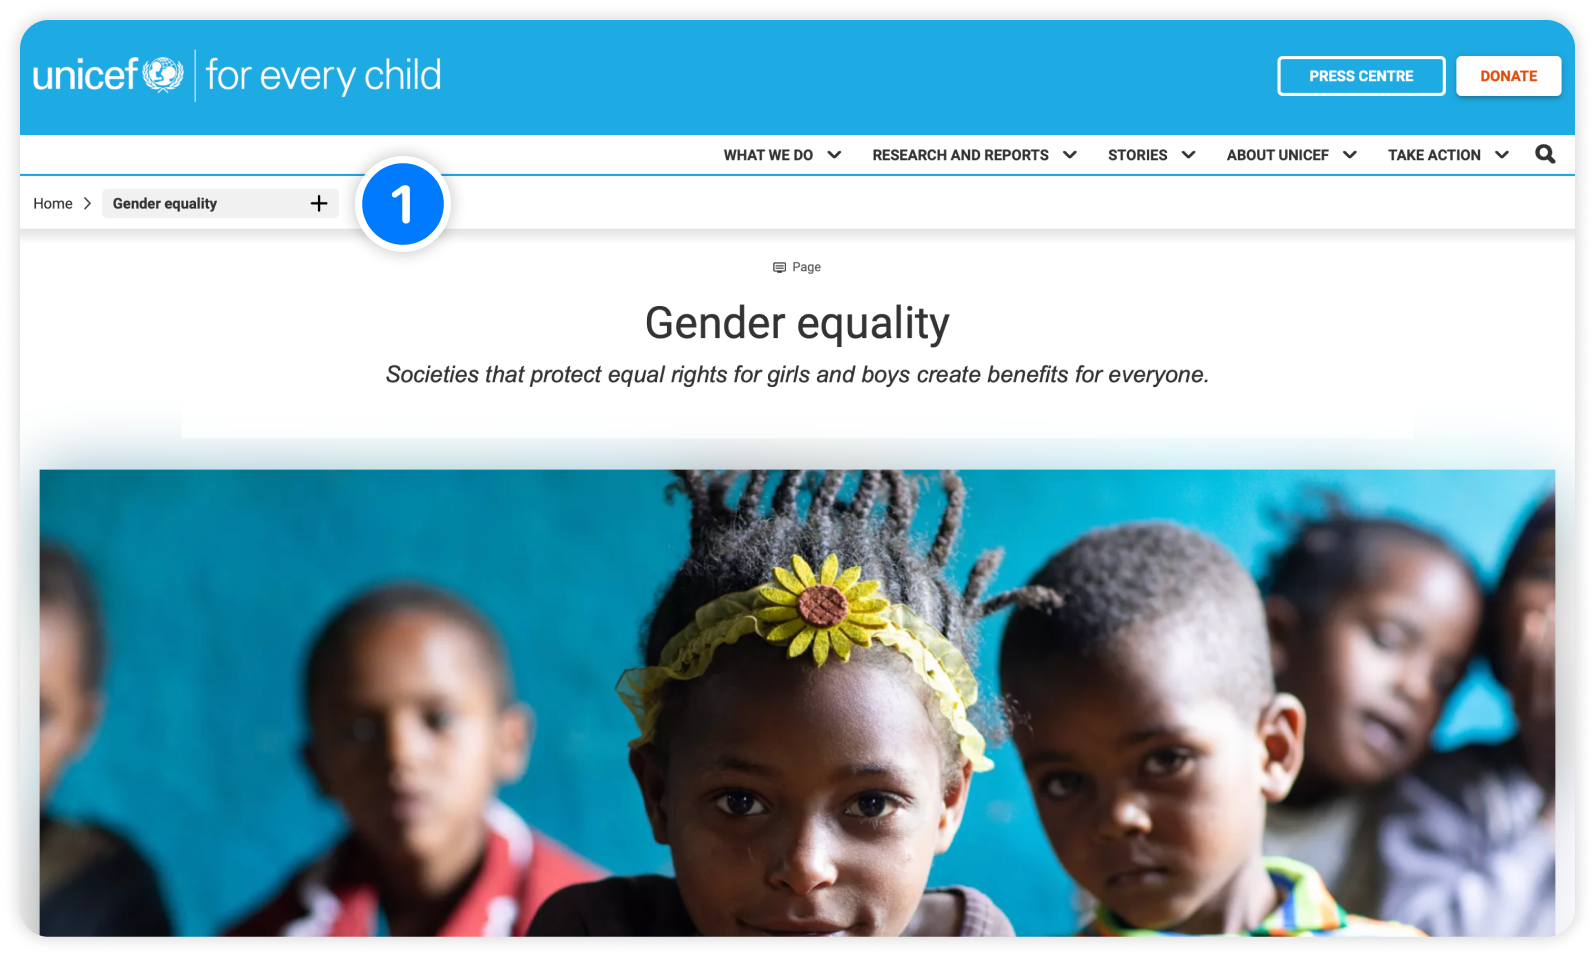
\includegraphics[scale=0.20]{Resources/Dario/breadcrumbs}
    \end{figure}
    \begin{figure}[h]
        \centering
        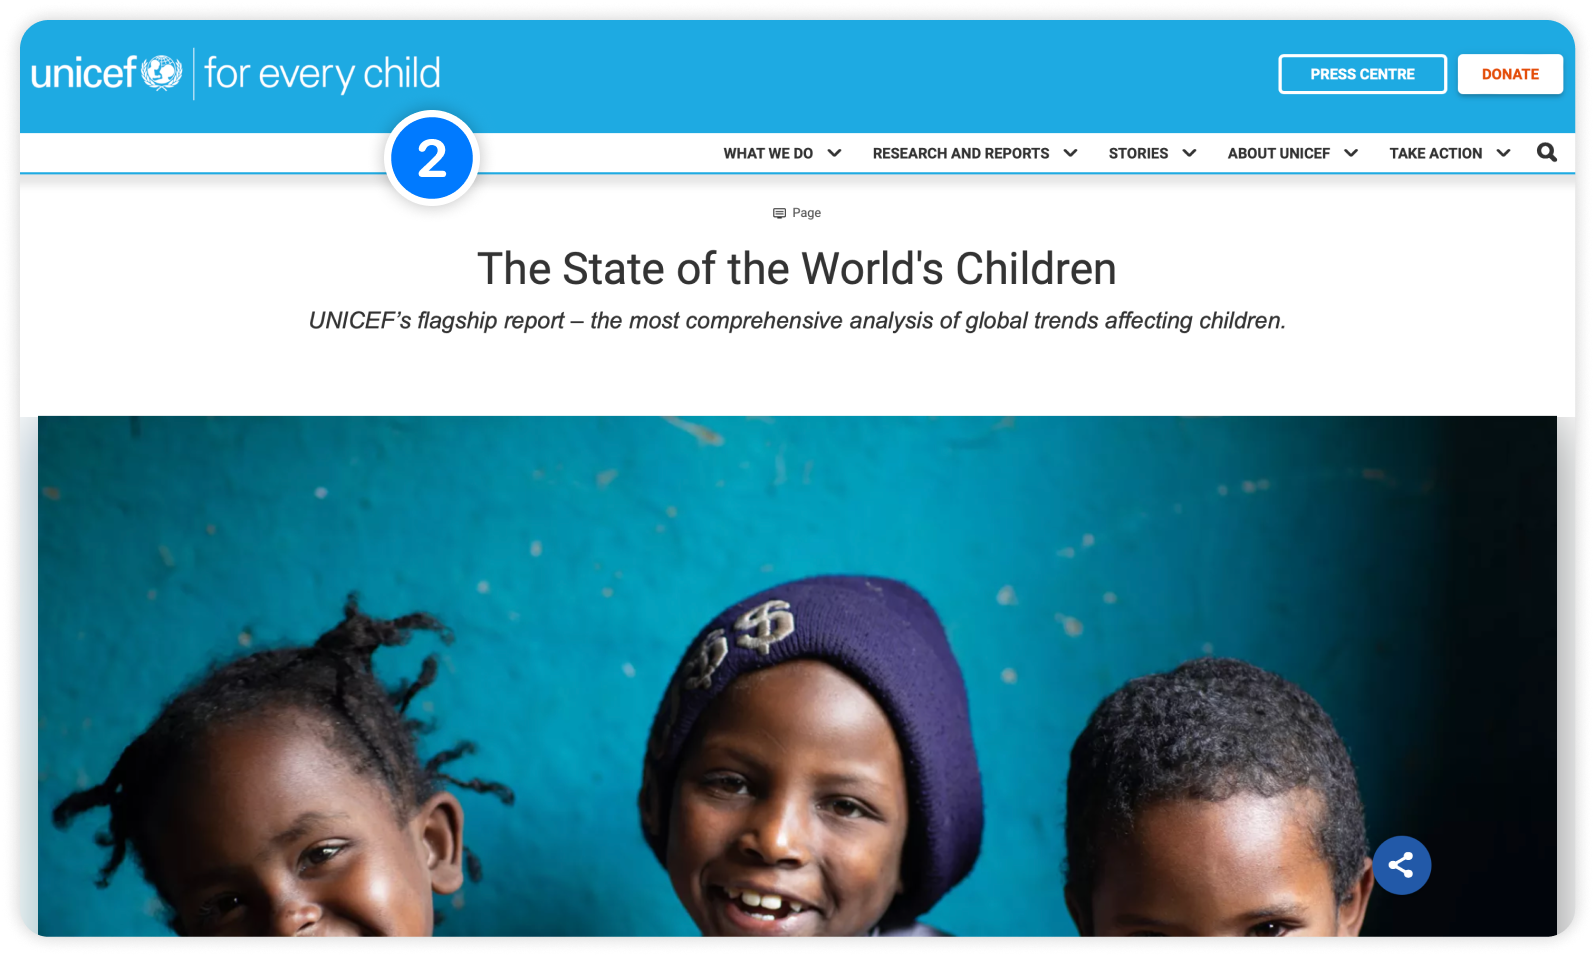
\includegraphics[scale=0.20]{Resources/Dario/nobreadcrumbs}
        \caption{Similar pages show different navigation logic}
    \end{figure}
    \item {\textbf{H2} \color{unicefGray}{Match between system and the real world}}\\
    The website effectively communicates in the users' native language and the organization of information is both logical and clear.
    \newpage
    \item {\textbf{H3} \color{unicefGray}{User control and freedom}}\\
    In the donation section an user is not able to modify the donation amount without losing the inserted personal information.
    \item {\textbf{H4} \color{unicefGray}{Consistency and standards}}\\
    All aspects are transparent and easily comprehensible devoid of any ambiguities.
    \item {\textbf{H5} \color{unicefGray}{Error prevention}}\\
    The website effectively guides users through the process of entering personal information in the donation section (1 and 3). 
    However, it remains possible for users to input meaningless information (2).
    Additionally a confirmation popup is triggered when a custom donation amount is entered.
    The user loses the inserted personal information if they decide to modify the donation amount (4).
    \begin{figure}[h]
        \centering
        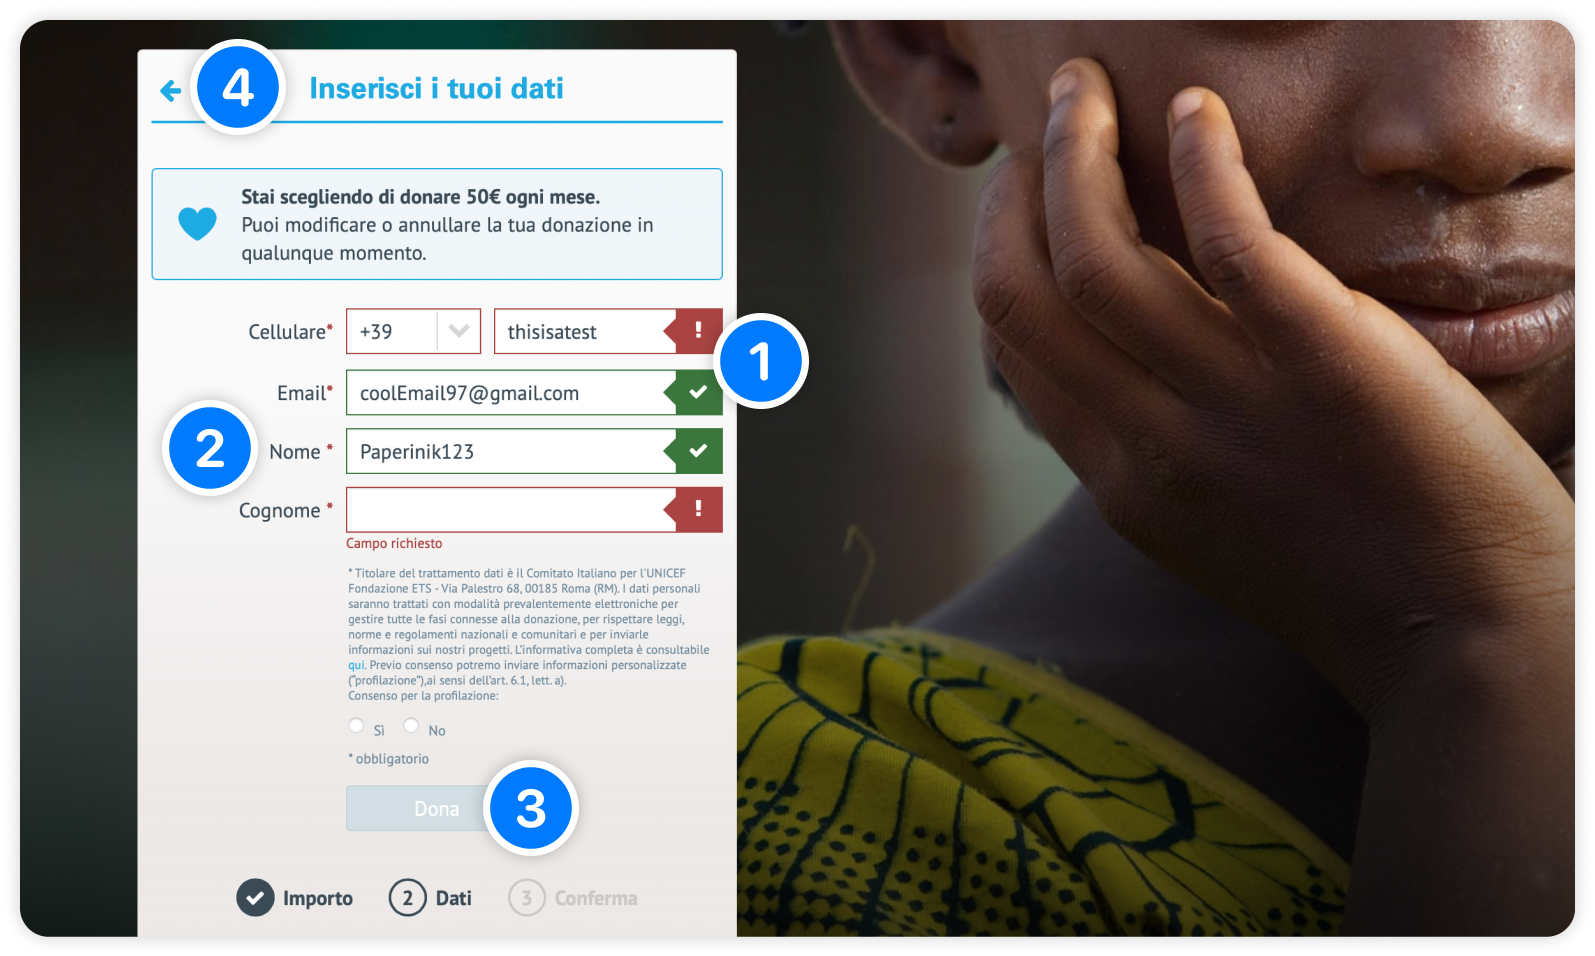
\includegraphics[scale=0.20]{Resources/Dario/donation}
        \caption{Error prevention in the donation section}
    \end{figure}
    \item {\textbf{H6} \color{unicefGray}{Recognition rather than recall}}\\
    Using the website proficiently requires no mnemonic work. It's designed for intuitive navigation and ease of use.
    \item {\textbf{H7} \color{unicefGray}{Flexibility and efficiency of use}}\\
    While the website offers shortcuts like the share button for quick sharing on major social media platforms, the navigation remains relatively static and there are no options for customization.
    \item {\textbf{H8} \color{unicefGray}{Aesthetic and minimalist design}}\\
    The website adopts a minimalistic approach, yet its aesthetic appeal may not be particularly pronounced. 
    Repetitions, such as the presence of multiple donation buttons on the page, are noticeable.
    \newpage
    \item {\textbf{H9} \color{unicefGray}{Help users recognize, diagnose and recover from errors}}\\
    This aspect cannot be tested deeply cause the website is essentially static and lacks of interactive features.
    \item {\textbf{H10} \color{unicefGray}{Help and documentation}}\\
    In the footer (1), users can access various links to gather useful information. 
    Both FAQs and documentation are available in multiple languages for enhanced accessibility.
    \begin{figure}[h]
        \centering
        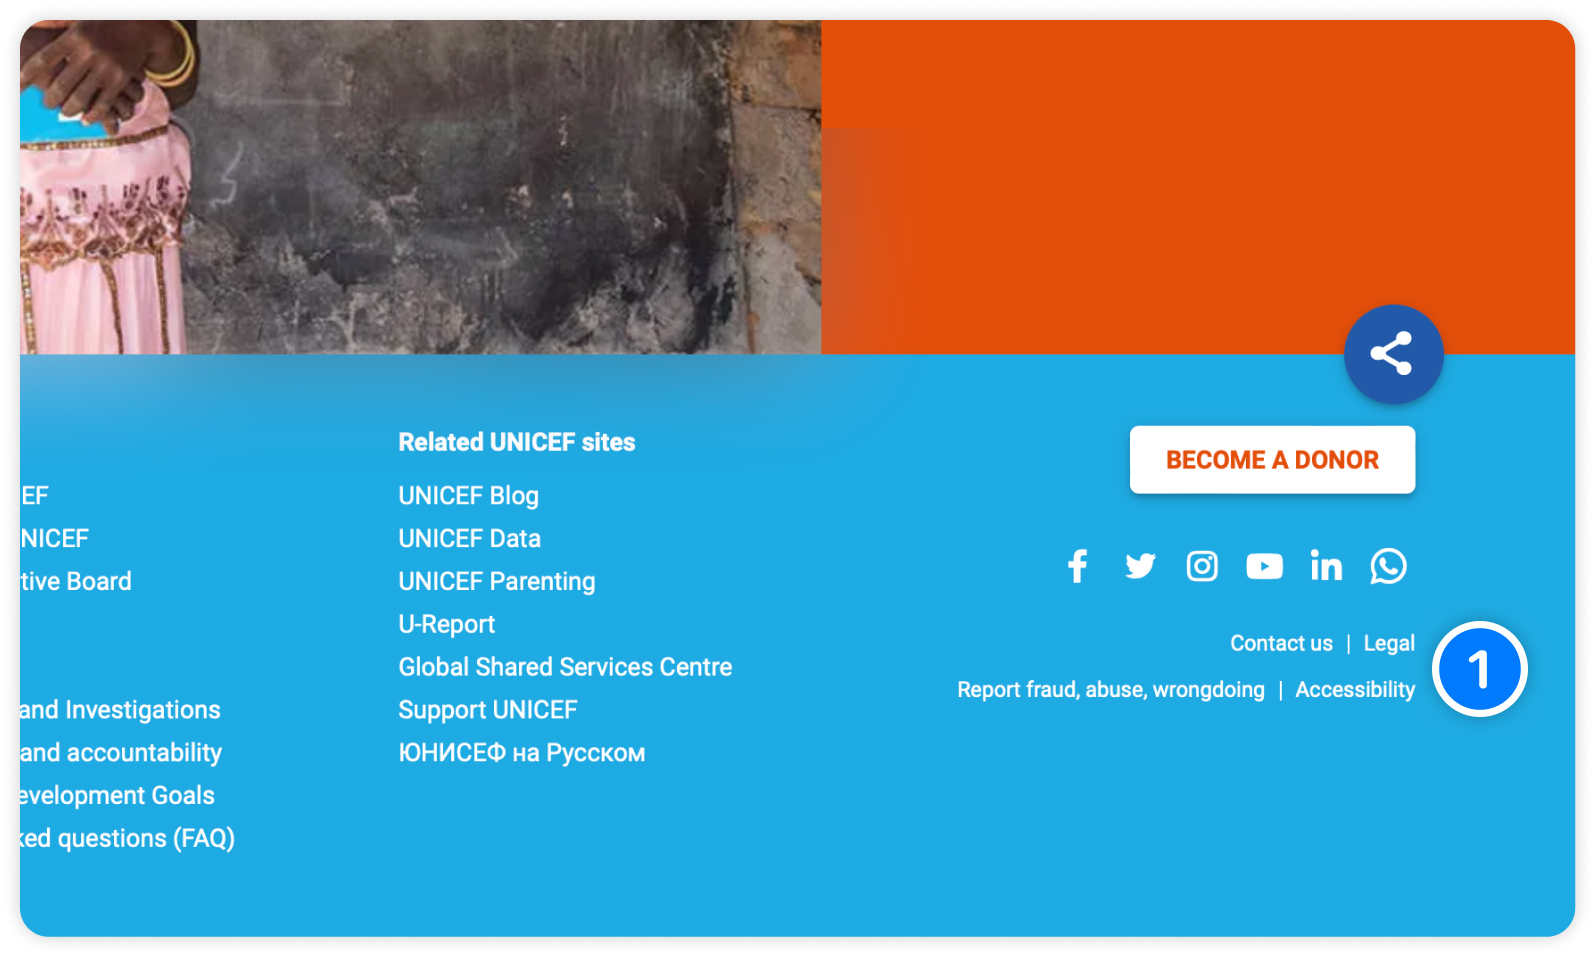
\includegraphics[scale=0.20]{Resources/Dario/footer}
        \caption{Useful links in the footer}
    \end{figure}
\end{description}
% MiLe Heuristics Comments
\newpage
\subsubsection{MiLe Heuristics}
\begin{description}
    \item {\textbf{M1} \color{unicefGray}{Interaction consistency}}\\
    Pages with similar content demonstrate varying navigation approaches
    \item {\textbf{M2} \color{unicefGray}{Group navigation}}\\
    Navigation throughout the website is seamless regardless of the user's position but the menus appear slightly overcrowded.
    \item {\textbf{M3} \color{unicefGray}{Navigation support}}\\
    Discovering the various components of a topic is straightforward.
    \item {\textbf{M4} \color{unicefGray}{User control}}\\
    While certain areas of the website excel in implementing interactive features others may feel somewhat unintuitive.
    \item {\textbf{M5} \color{unicefGray}{Error prevention}}\\
    Every section of the webpage is easily accessible through a simple and effective interface.
    \item {\textbf{M6} \color{unicefGray}{Information overload}}\\
    In certain sections or menus (1) the website may induce a sense of information overload.
    \begin{figure}[h]
        \centering
        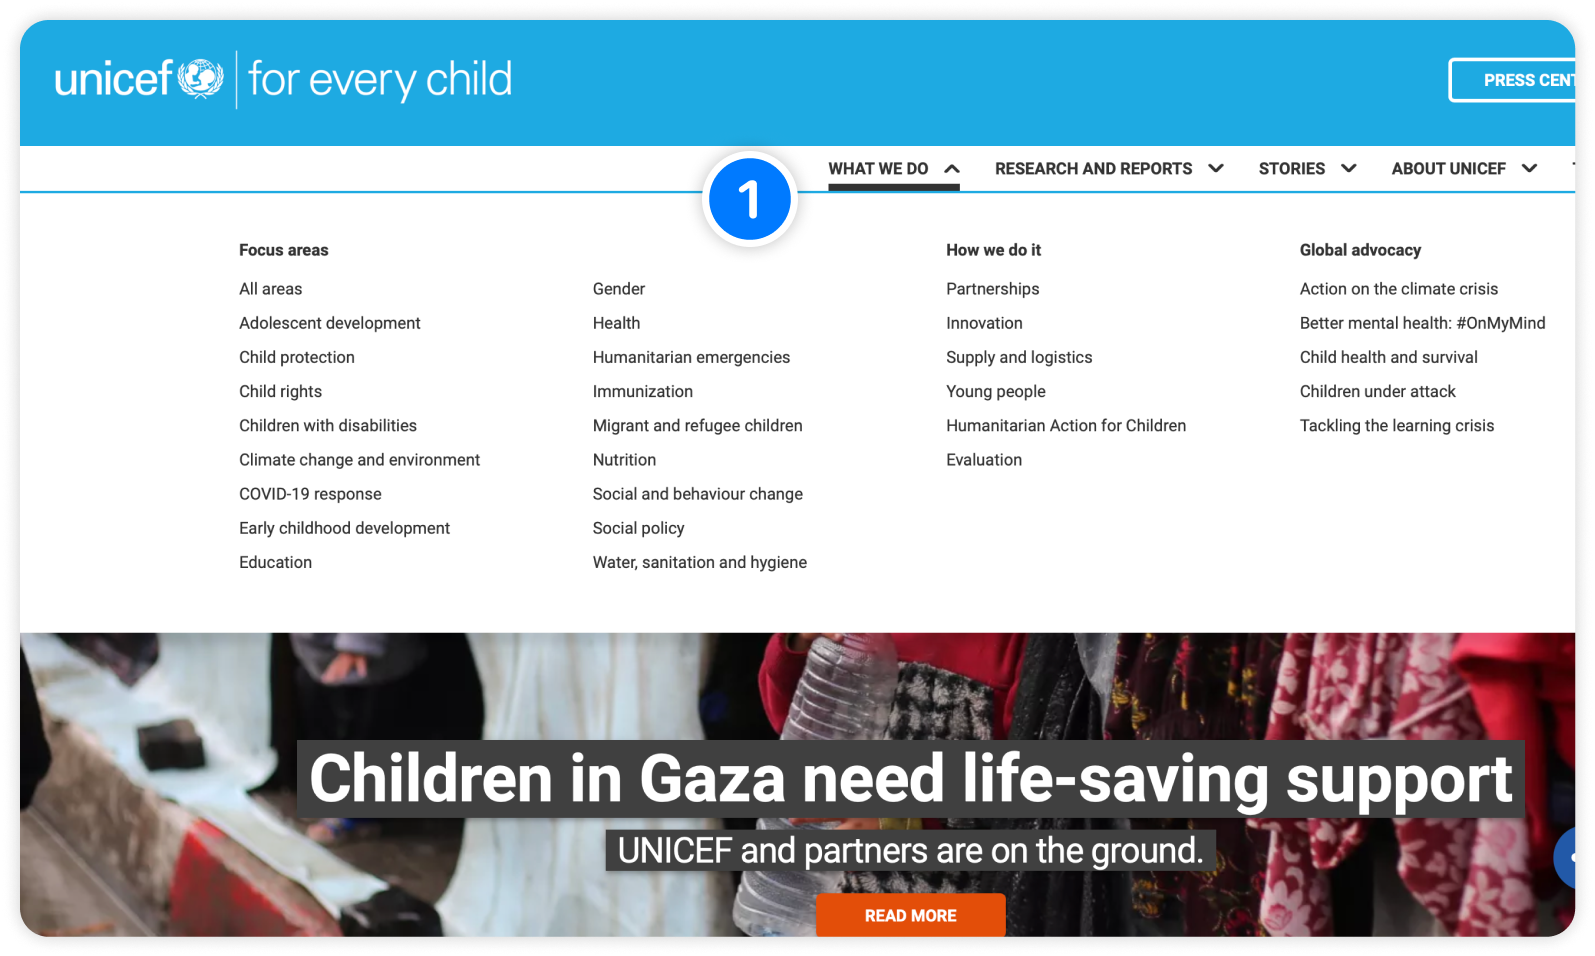
\includegraphics[scale=0.20]{Resources/Dario/menu}
        \caption{Some menus are a little bit overcrowded}
    \end{figure}
    \item {\textbf{M7} \color{unicefGray}{Text layout}}\\
    Nothing is left to chance in the text layout, with a clear and concise structure.
    \item {\textbf{M8} \color{unicefGray}{Interaction placeholder semiotics}}\\
    The website features a modest number of interactive elements, each conveying its functional purpose clearly and operating smoothly.
    \item {\textbf{M9} \color{unicefGray}{Interaction placeholder consistency}}\\
    The website maintains a consistent approach to interaction placeholders.
    \item {\textbf{M10} \color{unicefGray}{Spatial allocation}}\\
    I find the distribution of related elements on the page adequate, but personally, I believe that certain parts of the website require redesigning to enhance the user experience. 
    Overall, the website gives me a sense of overcrowding, suggesting that spatial organization could be improved to alleviate this issue.
    \item {\textbf{M11} \color{unicefGray}{Consistency of the page structure}}\\
    All pages adhere to a similar structure, with minor justified variations.
    \item {\textbf{M12} \color{unicefGray}{Coherence in page layout}}\\
    The website's layout is coherent and consistent, with a clear and logical structure.
\end{description}


